%% ============================================================
%%  Ligue 1 Match Prediction — Data Collection & Organisation
%%  Beamer presentation
%% ============================================================
\documentclass[aspectratio=169,12pt]{beamer}

%% ── Theme ────────────────────────────────────────────────────
\usetheme{Madrid}
\setbeamertemplate{navigation symbols}{}   % remove nav icons
\setbeamertemplate{footline}{%
  \leavevmode%
  \hbox{%
    \begin{beamercolorbox}[wd=.45\paperwidth,ht=2.4ex,dp=1ex,center]{author in head/foot}%
      \usebeamerfont{author in head/foot}\insertshortauthor
    \end{beamercolorbox}%
    \begin{beamercolorbox}[wd=.45\paperwidth,ht=2.4ex,dp=1ex,center]{title in head/foot}%
      \usebeamerfont{title in head/foot}\insertshorttitle
    \end{beamercolorbox}%
    \begin{beamercolorbox}[wd=.1\paperwidth,ht=2.4ex,dp=1ex,right]{date in head/foot}%
      \insertframenumber{}/\inserttotalframenumber\hspace*{2ex}
    \end{beamercolorbox}}%
}

%% ── Colours ──────────────────────────────────────────────────
\usepackage{xcolor}
\definecolor{darkblue}{RGB}{23,55,94}
\definecolor{midblue}{RGB}{44,123,182}
\definecolor{playercol}{RGB}{231,76,60}
\definecolor{fbrefcol}{RGB}{155,89,182}
\definecolor{understcol}{RGB}{44,123,182}
\definecolor{lightgrey}{RGB}{245,245,245}

\setbeamercolor{palette primary}{bg=darkblue,fg=white}
\setbeamercolor{palette secondary}{bg=midblue,fg=white}
\setbeamercolor{palette tertiary}{bg=darkblue,fg=white}
\setbeamercolor{frametitle}{bg=darkblue,fg=white}
\setbeamercolor{title}{fg=white}
\setbeamercolor{block title}{bg=midblue,fg=white}
\setbeamercolor{block body}{bg=lightgrey,fg=black}
\setbeamercolor{alerted text}{fg=playercol}

%% ── Packages ─────────────────────────────────────────────────
\usepackage{graphicx}
\usepackage{booktabs}
\usepackage{tabularx}
\usepackage{tikz}
\usetikzlibrary{arrows.meta,shapes.geometric,positioning,calc}
\usepackage{fontawesome5}
\usepackage{array}
\usepackage{multirow}
\usepackage{amsmath}

%% ── Metadata ─────────────────────────────────────────────────
\title[Player-Level Match Prediction]{%
  Predicting Ligue 1 Match Outcomes\\
  with Player-Level Statistics}
\subtitle{Data Collection \& Feature Organisation}
\author[S.\ O'Shea]{Sienna O'Shea}
\date{}

%% ═══════════════════════════════════════════════════════════
\begin{document}

%% ── Title slide ─────────────────────────────────────────────
{
\setbeamertemplate{footline}{}
\begin{frame}
  \titlepage
  \vspace{-0.8em}
  \begin{center}
    \small Ligue 1 · Seasons 2018--2024 · 1{,}653 matches · 73 features
  \end{center}
\end{frame}
}

%% ── Outline ─────────────────────────────────────────────────
\begin{frame}{Outline}
  \tableofcontents
\end{frame}

%% ═══════════════════════════════════════════════════════════
\section{Research Hypothesis}
%% ═══════════════════════════════════════════════════════════

\begin{frame}{Central Hypothesis}
  \begin{block}{Research Question}
    Do \alert{player-level} rolling statistics add predictive power
    for match outcomes beyond team-level aggregates and bookmaker odds?
  \end{block}

  \vspace{0.6em}

  \begin{columns}[T]
    \column{0.48\textwidth}
    \textbf{Standard approach}\\[0.4em]
    Team-level rolling form $\cdot$ squad market value $\cdot$
    bookmaker implied probabilities

    \column{0.48\textwidth}
    \textbf{This project adds}\\[0.4em]
    Per-player rolling stats \emph{tracked across transfers},
    aggregated over the starting XI weighted by minutes played
  \end{columns}

  \vspace{0.6em}

  \begin{alertblock}{Key insight}
    Tracking individual player form (not team form) captures information
    like mid-season transfers, rotation, and injury recovery that team
    aggregates smooth over.
  \end{alertblock}
\end{frame}

%% ═══════════════════════════════════════════════════════════
\section{Data Sources}
%% ═══════════════════════════════════════════════════════════

\begin{frame}{Data Sources — Three Pipelines}
  \begin{columns}[T]

    \column{0.32\textwidth}
    \begin{block}{\textcolor{understcol}{\faDatabase}\; Understat}
      \small
      \textbf{What:} xG timelines, match results, pre-match win/draw/loss
      probabilities\\[0.3em]
      \textbf{Seasons:} 2018--2023\\[0.3em]
      \textbf{Rows:} 2{,}105 matches\\[0.3em]
      \textbf{Script:} \texttt{collect\_understat.py}
    \end{block}

    \column{0.32\textwidth}
    \begin{block}{\textcolor{fbrefcol}{\faDatabase}\; Transfermarkt}
      \small
      \textbf{What:} Squad market values, player counts, squad age\\[0.3em]
      \textbf{Seasons:} 2018--2023\\[0.3em]
      \textbf{Rows:} 174 team-seasons\\[0.3em]
      \textbf{Script:} \texttt{collect\_transfermarkt.py}
    \end{block}

    \column{0.32\textwidth}
    \begin{block}{\textcolor{playercol}{\faDatabase}\; FBref}
      \small
      \textbf{What:} Per-player per-match: goals, assists, shots, SoT,
      tackles, interceptions, minutes, position\\[0.3em]
      \textbf{Rows:} 62{,}683 player-match rows\\[0.3em]
      \textbf{Script:} \texttt{collect\_fbref.py}
    \end{block}

  \end{columns}

  \vspace{0.5em}
  \small
  FBref data was scraped via \texttt{soccerdata} using an undetected
  headless Chrome driver; the 2021/22 season required a visible browser
  pass to resolve a CAPTCHA block.
\end{frame}

%% ── Pipeline diagram ─────────────────────────────────────────
\begin{frame}{Data Pipeline}
\begin{center}
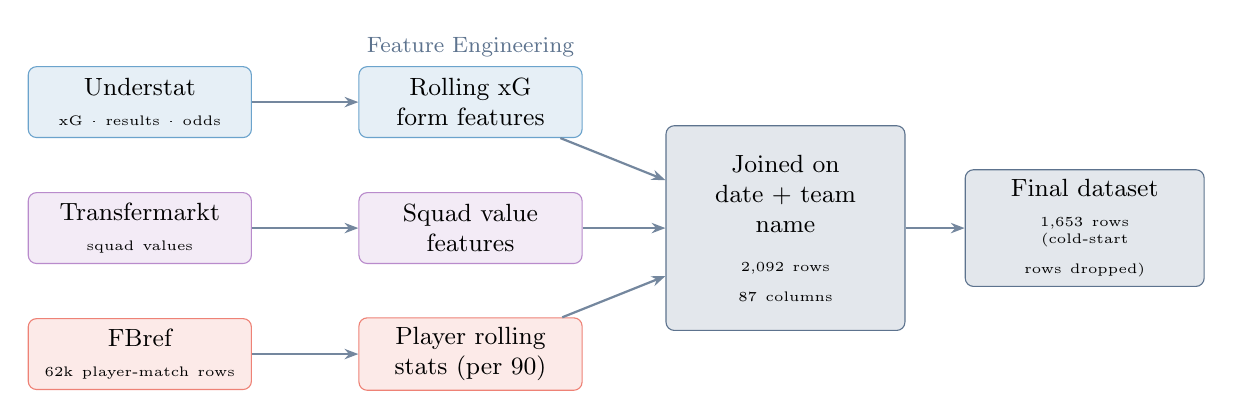
\begin{tikzpicture}[
  boxu/.style={rectangle, rounded corners=3pt, draw=understcol!70, fill=understcol!12,
               text width=2.6cm, align=center, minimum height=0.9cm, font=\small},
  boxf/.style={rectangle, rounded corners=3pt, draw=fbrefcol!70,   fill=fbrefcol!12,
               text width=2.6cm, align=center, minimum height=0.9cm, font=\small},
  boxp/.style={rectangle, rounded corners=3pt, draw=playercol!70,  fill=playercol!12,
               text width=2.6cm, align=center, minimum height=0.9cm, font=\small},
  boxd/.style={rectangle, rounded corners=3pt, draw=darkblue!70,   fill=darkblue!12,
               text width=2.8cm, align=center, minimum height=0.9cm, font=\small},
  arr/.style={-{Stealth[length=5pt]}, thick, color=darkblue!60},
  lbl/.style={font=\footnotesize, color=darkblue!70}
]

%% sources
\node[boxu] (us)  at (0,0)   {Understat\\{\tiny xG · results · odds}};
\node[boxf] (tm)  at (0,-1.6){Transfermarkt\\{\tiny squad values}};
\node[boxp] (fb)  at (0,-3.2){FBref\\{\tiny 62k player-match rows}};

%% engineering
\node[boxu] (fe1) at (4.2, 0)   {Rolling xG\\form features};
\node[boxf] (fe2) at (4.2,-1.6) {Squad value\\features};
\node[boxp] (fe3) at (4.2,-3.2) {Player rolling\\stats (per 90)};

%% join
\node[boxd, text width=2.8cm, minimum height=2.6cm]
      (join) at (8.2,-1.6) {Joined on\\date + team\\name\\[0.3em]{\tiny 2{,}092 rows}\\{\tiny 87 columns}};

%% final
\node[boxd] (final) at (12,-1.6)
  {Final dataset\\{\tiny 1{,}653 rows}\\{\tiny (cold-start\\rows dropped)}};

\draw[arr] (us)  -- (fe1);
\draw[arr] (tm)  -- (fe2);
\draw[arr] (fb)  -- (fe3);
\draw[arr] (fe1) -- (join);
\draw[arr] (fe2) -- (join);
\draw[arr] (fe3) -- (join);
\draw[arr] (join) -- (final);

\node[lbl, above=0pt of fe1] {Feature Engineering};
\end{tikzpicture}
\end{center}
\end{frame}

%% ═══════════════════════════════════════════════════════════
\section{Dataset Overview}
%% ═══════════════════════════════════════════════════════════

\begin{frame}{Dataset at a Glance}
  \begin{columns}[T]
    \column{0.38\textwidth}
    \begin{block}{Coverage}
      \small
      \begin{tabular}{ll}
        Matches   & 1{,}653 \\
        Seasons   & 2018--2024 \\
        Teams     & 29 (incl.\ promoted) \\
        Features  & 73 \\
        Target    & H / D / A \\
      \end{tabular}
    \end{block}

    \vspace{0.4em}

    \begin{block}{Feature sources}
      \small
      \begin{tabular}{lr}
        Understat / Transfermarkt & 32 \\
        FBref team-level          & 17 \\
        \alert{Player-level}      & 24 \\
      \end{tabular}
    \end{block}

    \column{0.58\textwidth}
    \begin{block}{Season breakdown}
      \small
      \begin{tabular}{llp{3.4cm}}
        \toprule
        Season & Matches & Note \\
        \midrule
        2018/19 & 370 & \\
        2019/20 & 278 & COVID — curtailed \\
        2020/21 & 379 & \\
        2021/22 & 379 & FBref initially blocked \\
        2022/23 & 380 & \\
        2023/24 & 306 & Partial (to May 2024) \\
        \bottomrule
      \end{tabular}
    \end{block}
  \end{columns}
\end{frame}

%% ── Plot 1: target distribution ─────────────────────────────
\begin{frame}{Plot 1 — Target Variable Distribution}
  \begin{center}
    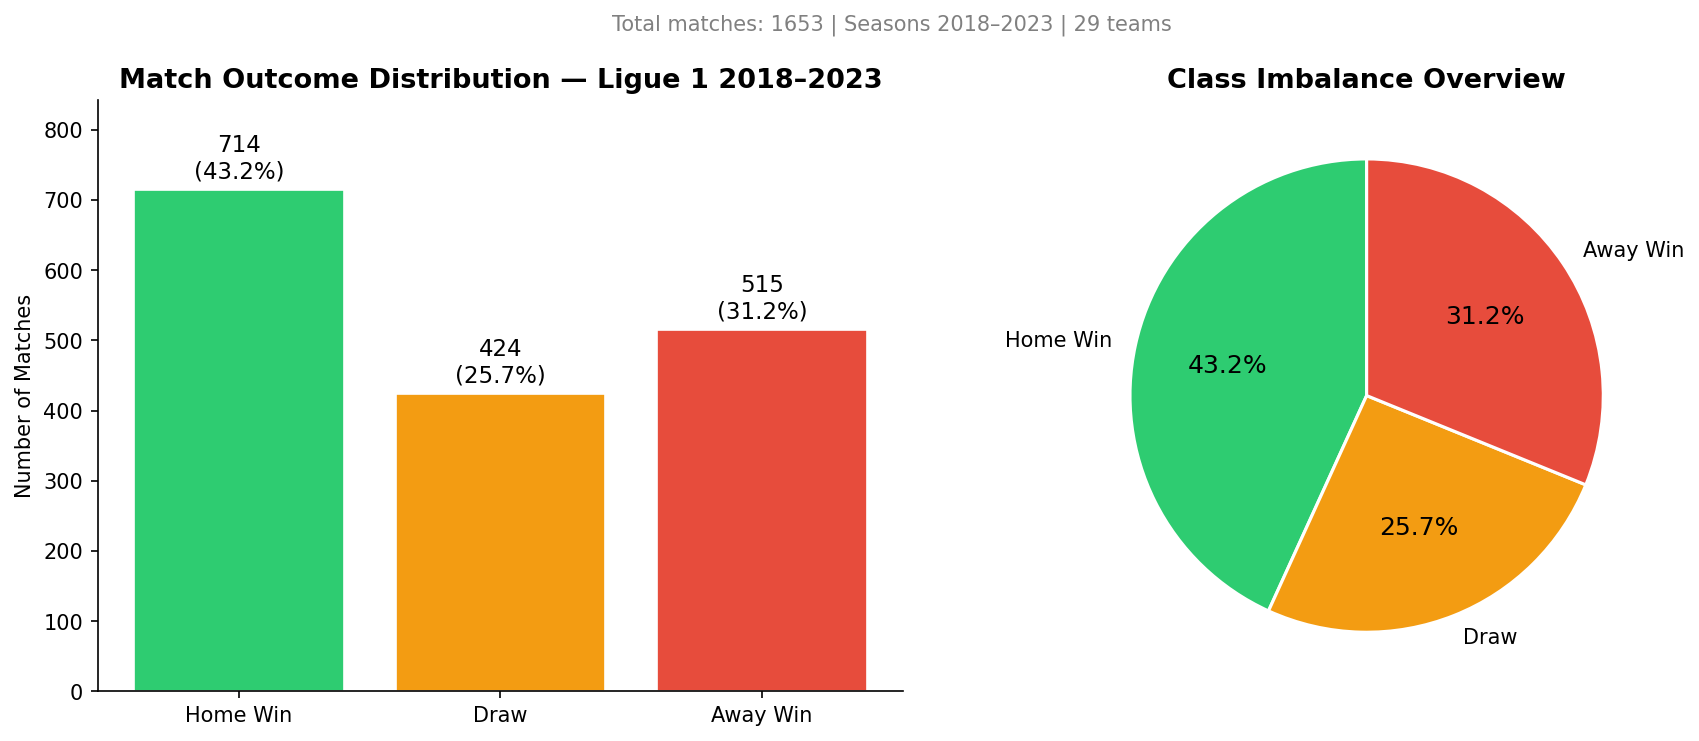
\includegraphics[width=0.75\textwidth]{../outputs/eda/01_target_distribution.png}
  \end{center}
  \begin{alertblock}{\small Class imbalance}
    \small Draws are underrepresented at $\approx$26\%.
    Models must use class weights or calibrated probabilities —
    accuracy alone is a misleading metric.
  \end{alertblock}
\end{frame}

%% ── Plot 3: missing data ─────────────────────────────────────
\begin{frame}{Plot 3 — Missing Data: Sources \& Resolution}
  \begin{center}
    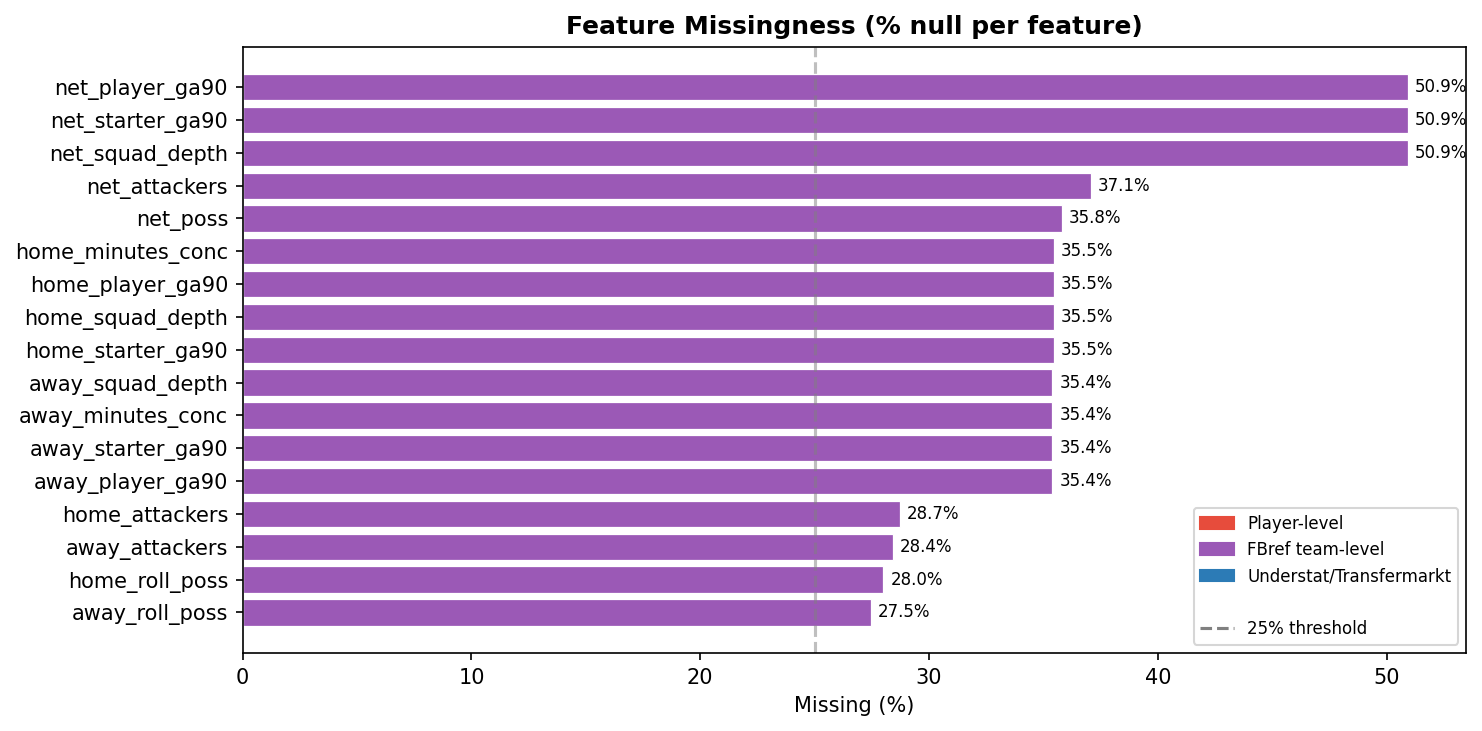
\includegraphics[width=0.68\textwidth]{../outputs/eda/03_missingness.png}
  \end{center}
  \vspace{0.2em}
  \footnotesize
  \begin{columns}[T]
    \column{0.48\textwidth}
    \textbf{FBref team features ($\sim$28--36\% null):} possession and
    formation data for 2021/22 was not scraped — FBref blocked that season.
    Handled via imputation.

    \column{0.48\textwidth}
    \textbf{Player rolling stats:} cold-start nulls (first $\approx$3
    matchdays/season). Fixed by dropping those 439 rows, leaving
    1{,}653 clean matches.
  \end{columns}
\end{frame}

%% ═══════════════════════════════════════════════════════════
\section{Feature Engineering}
%% ═══════════════════════════════════════════════════════════

\begin{frame}{Feature Engineering — Three Stages}
  \begin{block}{Stage 1 — Understat + Transfermarkt}
    \footnotesize Rolling 5-match xG, goals, wins, points per team.
    Squad market value, average player value, squad age.
    Bookmaker implied win/draw/loss probabilities.
  \end{block}

  \vspace{0.15em}

  \begin{block}{Stage 2 — FBref team-level}
    \footnotesize Rolling possession, formation (attackers count),
    player season G$+$A/90 aggregated to team level.
  \end{block}

  \vspace{0.15em}

  \begin{alertblock}{Stage 3 — Player-level (novel contribution)}
    \footnotesize Per-player rolling shots, SoT, defensive actions, goals, assists per 90
    tracked \emph{across team changes}.
    Aggregated over the starting XI weighted by minutes played.
    Net differentials (home $-$ away) for each stat.
  \end{alertblock}

  \vspace{0.2em}
  \footnotesize All rolling windows use \texttt{shift(1)} before rolling mean —
  the current match is \emph{never} included in its own features.
\end{frame}

\begin{frame}{Player-Level Aggregation Logic}
  \begin{columns}[T]
    \column{0.5\textwidth}
    \textbf{Per player, prior 5 appearances:}
    \[
      \text{roll}_{p,t} = \frac{1}{5}\sum_{k=1}^{5} \text{stat}_{p,t-k}
    \]
    Tracked \emph{individually} — a transfer does not reset form.

    \vspace{0.7em}

    \textbf{Starting XI aggregate (weighted mean):}
    \[
      \hat{s}_{\text{team}} = \frac{\sum_{p \in \text{XI}} \text{min}_p \cdot \text{roll}_{p}}{\sum_{p \in \text{XI}} \text{min}_p}
    \]

    \column{0.46\textwidth}
    \begin{block}{Player features produced}
      \small
      \begin{tabular}{ll}
        \texttt{*\_sh\_p90}       & shots / 90 \\
        \texttt{*\_sot\_p90}      & shots on target / 90 \\
        \texttt{*\_def\_p90}      & TklW $+$ Int / 90 \\
        \texttt{*\_gls\_p90}      & goals / 90 \\
        \texttt{*\_ast\_p90}      & assists / 90 \\
        \texttt{*\_starter\_mins} & regularity proxy \\
        \texttt{*\_pct\_fw}       & fraction forwards \\
        \texttt{*\_depth\_sh}     & shot depth gap \\
      \end{tabular}\\[0.3em]
      Each exists as \texttt{home\_pl\_*},
      \texttt{away\_pl\_*}, \texttt{net\_pl\_*}
    \end{block}
  \end{columns}
\end{frame}

%% ═══════════════════════════════════════════════════════════
\section{Feature Selection}
%% ═══════════════════════════════════════════════════════════

\begin{frame}{Feature Selection — Four-Method Protocol}
  \footnotesize Each of the 73 features was scored by \textbf{four independent methods},
  percentile-normalised (0--1), and averaged into a \textbf{composite score}.

  \vspace{0.25em}

  \begin{columns}[T]
    \column{0.48\textwidth}
    \begin{block}{1. Mutual Information (Filter)}
      \footnotesize How much does knowing this feature reduce uncertainty about the result?
      Non-parametric; catches non-linear relationships.
    \end{block}
    \vspace{0.15em}
    \begin{block}{2. RFECV — Wrapper}
      \footnotesize A Random Forest eliminates weak features iteratively under
      temporal CV. Only features it \emph{keeps} survive.
      Optimal: \textbf{26 features}.
    \end{block}

    \column{0.48\textwidth}
    \begin{block}{3. LASSO (Embedded)}
      \footnotesize Penalised logistic regression zeroes redundant features.
      17 features zeroed; \textbf{0 player features} zeroed.
    \end{block}
    \vspace{0.15em}
    \begin{block}{4. RF Importance (Embedded)}
      \footnotesize Mean decrease in impurity across 300 trees.
      Stable across seeds; corroborates RFECV ranking.
    \end{block}
  \end{columns}

  \vspace{0.2em}
  \footnotesize\textit{Temporal CV (TimeSeriesSplit, 5 folds) throughout — data never shuffled across time.}
\end{frame}

%% ── Plot 4: feature distributions ───────────────────────────
\begin{frame}{Plot 4 — Feature Distributions by Match Outcome (Top 20)}
  \begin{columns}[T]
    \column{0.50\textwidth}
    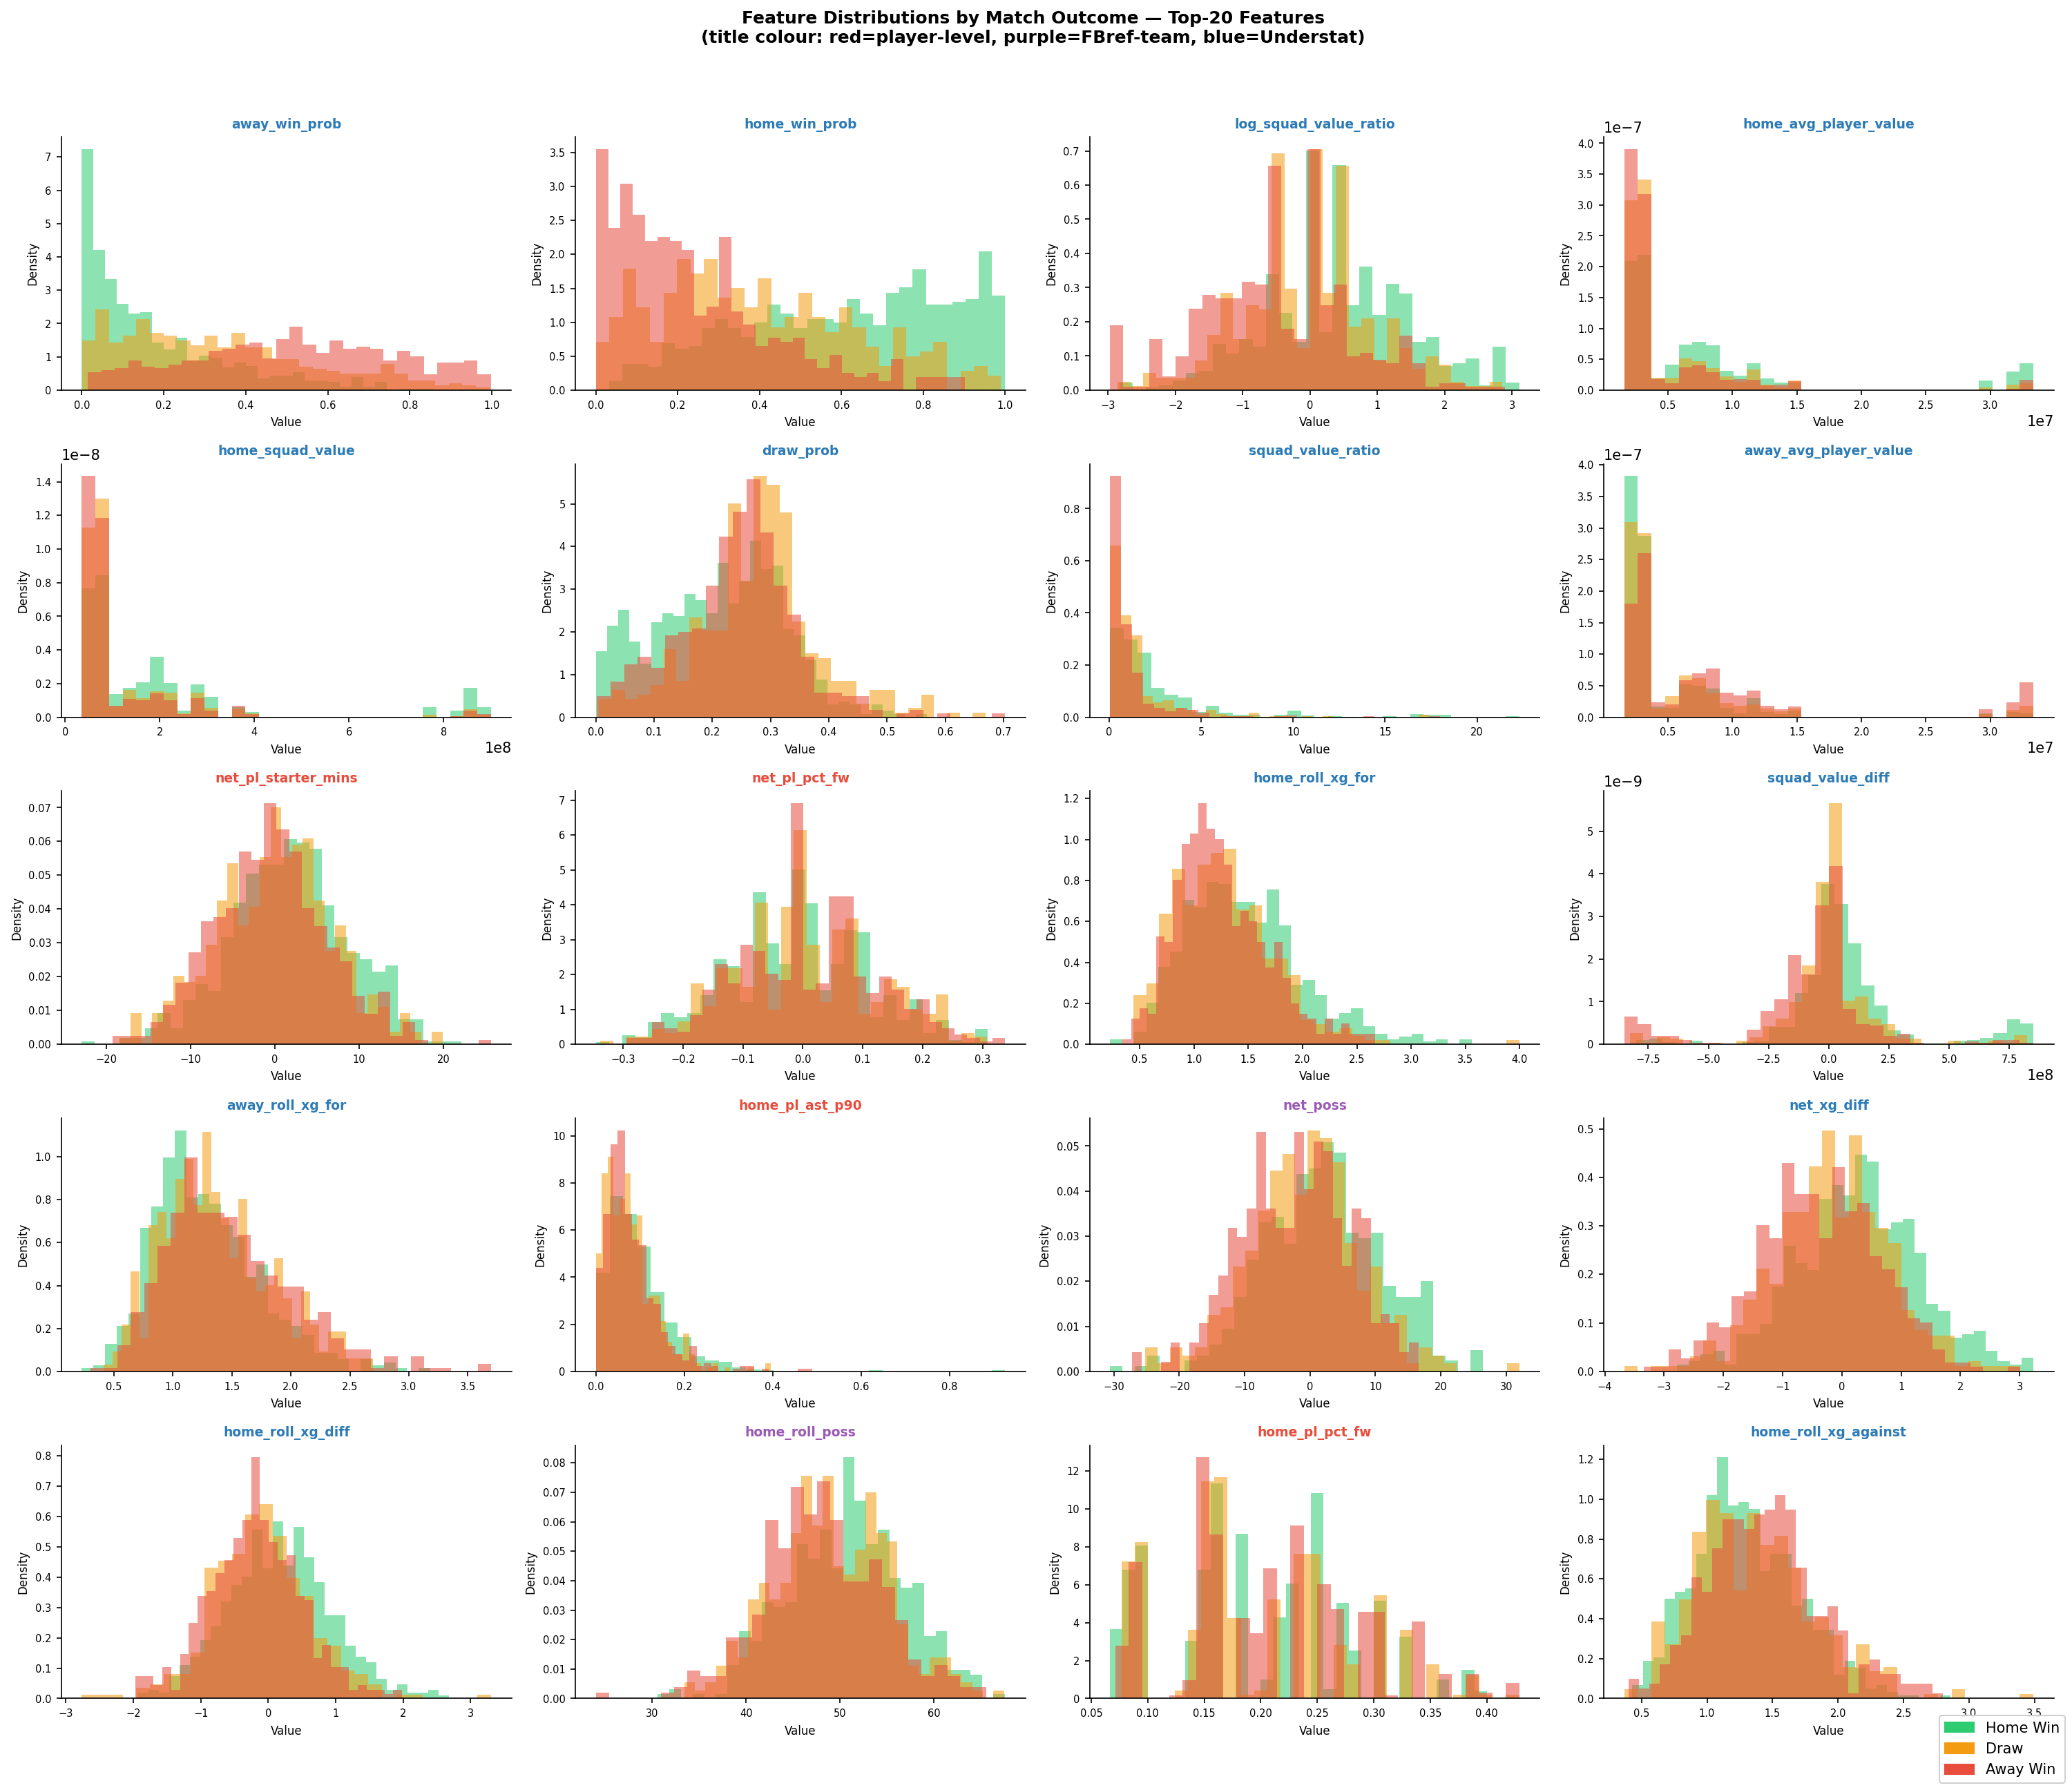
\includegraphics[width=\linewidth]{../outputs/eda/04_histograms_by_result.png}

    \column{0.47\textwidth}
    \vspace{0.5em}
    \small\textbf{How to read:} each panel shows the distribution of one
    feature split by match outcome (H/D/A).

    \vspace{0.6em}
    \textbf{Less overlap} between the three coloured distributions
    $\Rightarrow$ more discriminative feature.

    \vspace{0.6em}
    \textcolor{understcol}{\textbf{Bookmaker probability features}} show the
    clearest separation.

    \vspace{0.6em}
    \textcolor{playercol}{\textbf{Player-level features}} add a small but
    consistent nudge on top of the bookmaker signal.
  \end{columns}
\end{frame}

%% ── Plot 8: bookmaker vs player cross-correlation ────────────
\begin{frame}{Plot 8 — Bookmaker Odds vs Player-Level Features}
  \begin{center}
    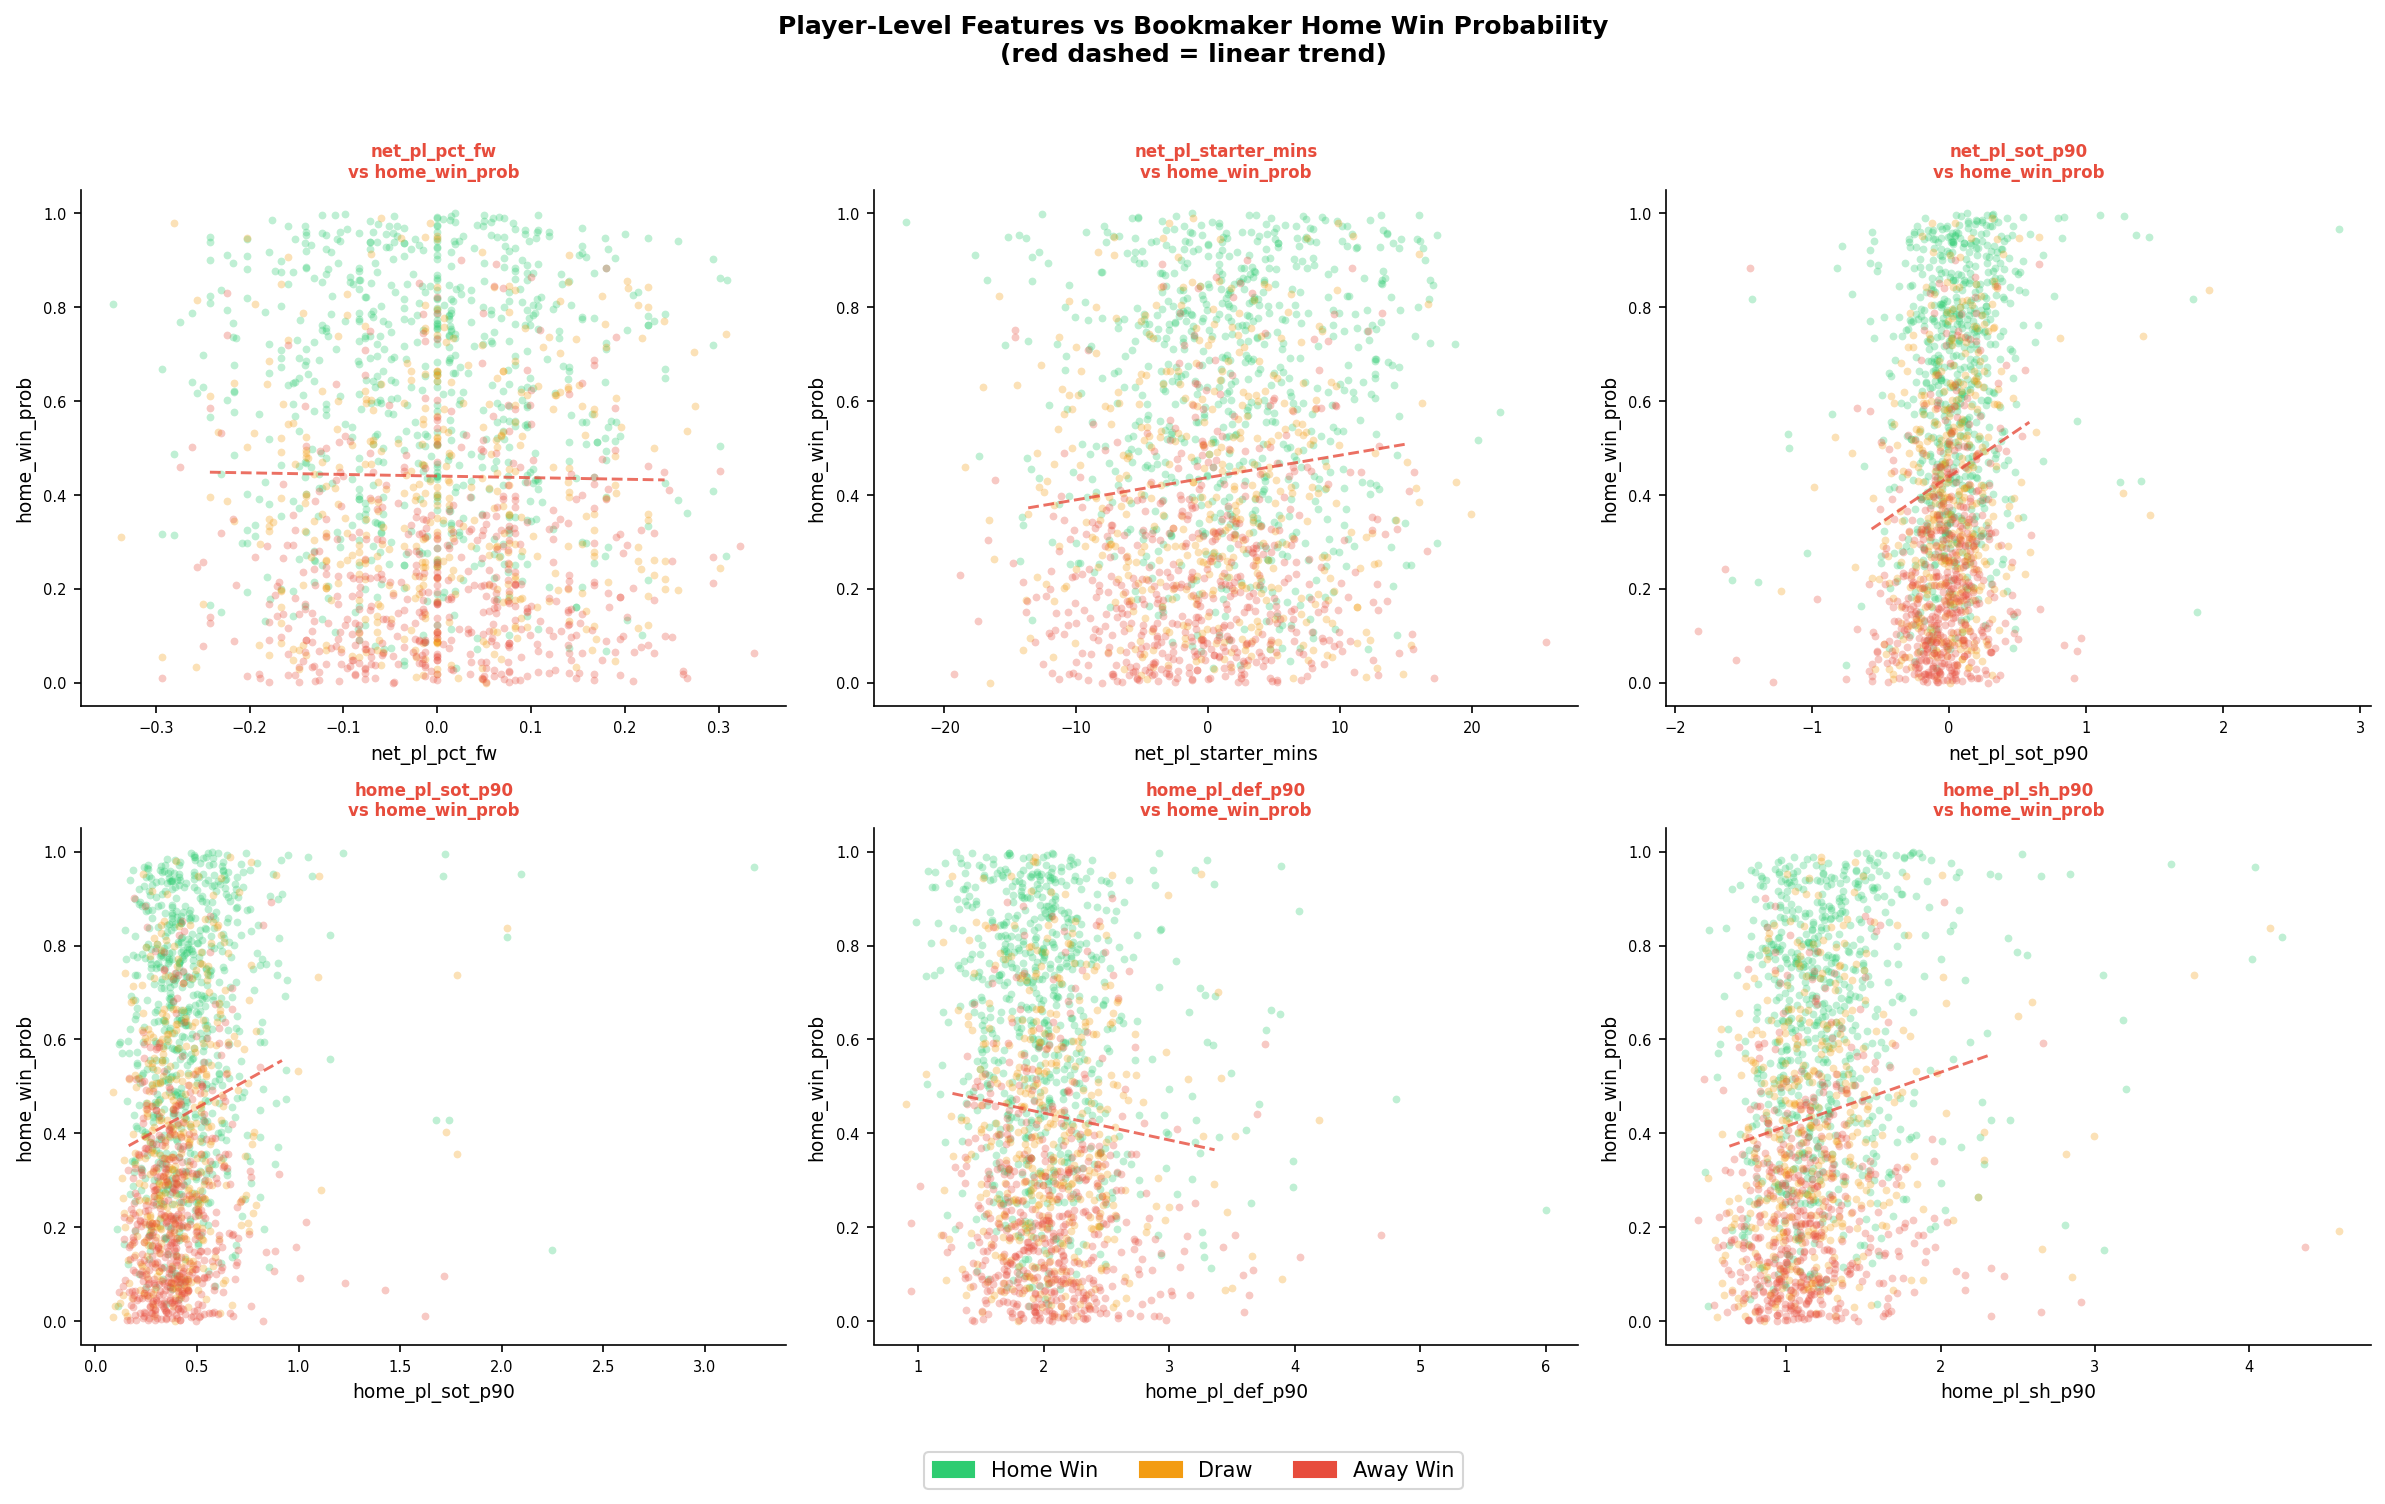
\includegraphics[width=0.58\textwidth]{../outputs/eda/08_player_features_vs_bookmaker.png}
  \end{center}
  \vspace{0.2em}
  \small
  The bookmaker's implied probability and the player rolling stats
  \textbf{mostly disagree} — wide scatter, no tight trend.
  This is a good sign: player features are contributing
  \emph{new information} that the bookmaker does not fully price in.
\end{frame}

%% ── Plot 12: feature leaderboard ─────────────────────────────
\begin{frame}{Plot 12 — Feature Leaderboard: All 73 Features Ranked}
  \begin{center}
    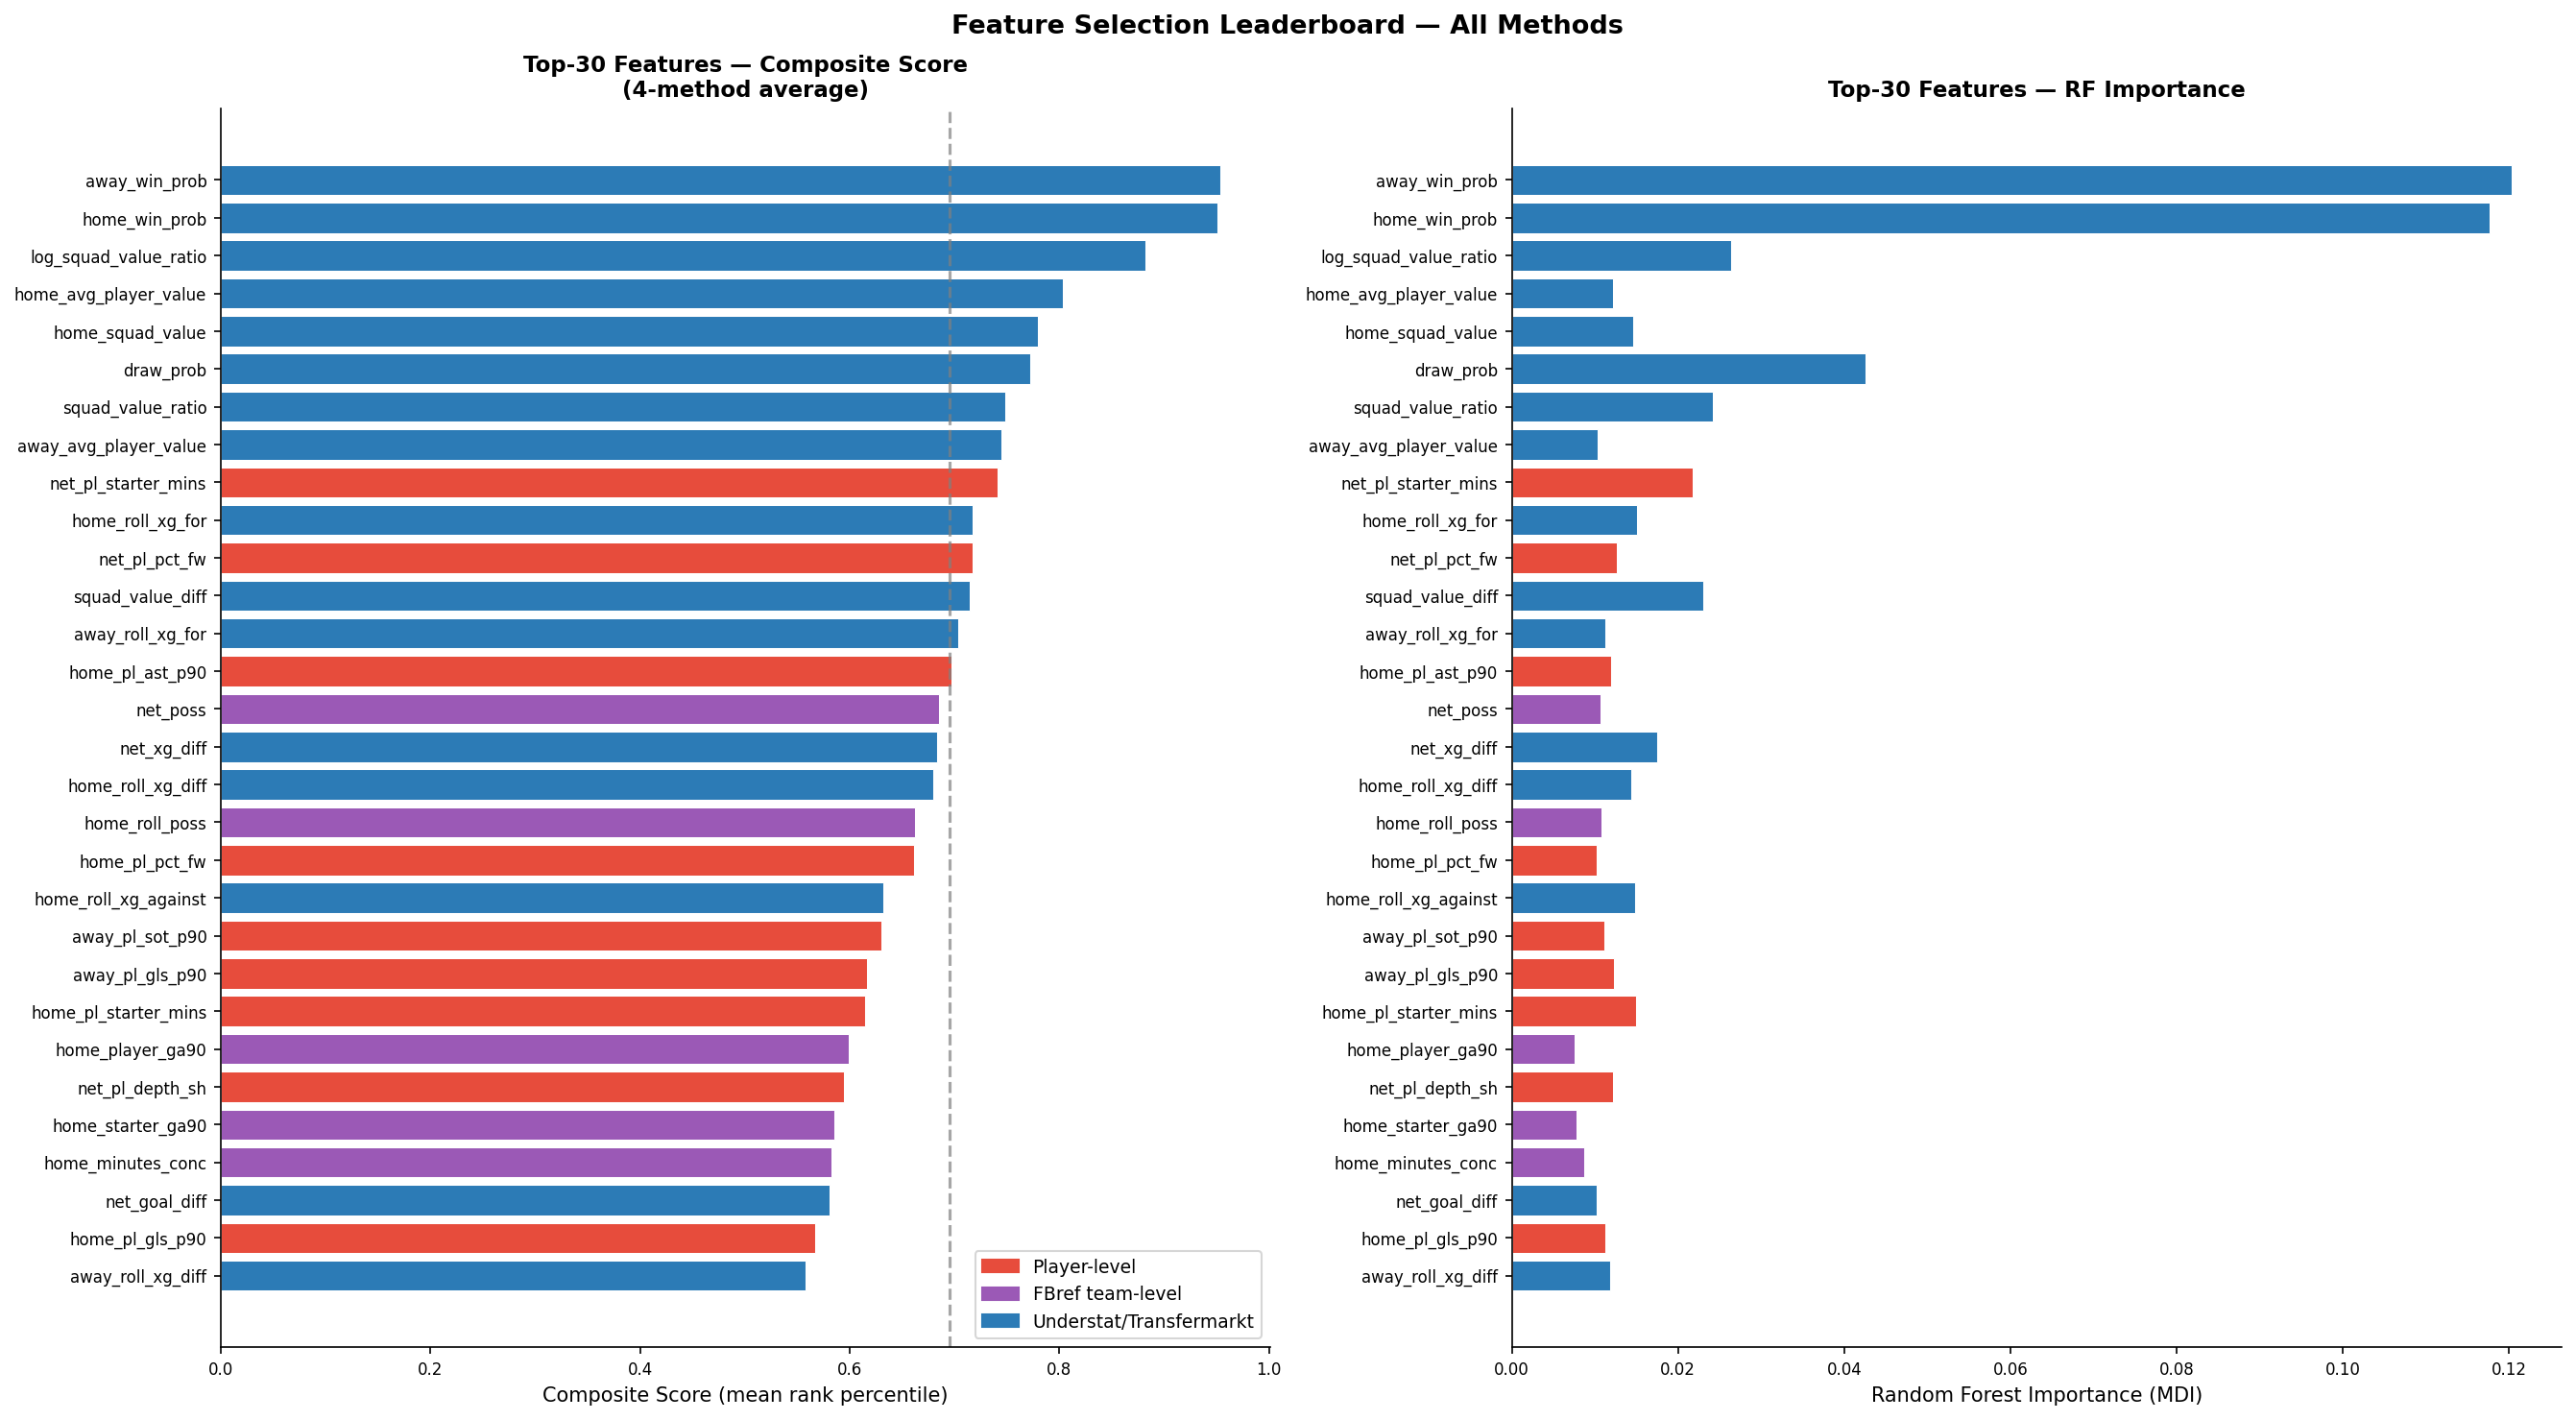
\includegraphics[width=0.64\textwidth]{../outputs/eda/12_feature_leaderboard_summary.png}
  \end{center}
  \vspace{0.1em}
  \small
  \textcolor{understcol}{$\blacksquare$ Understat/Transfermarkt}\quad
  \textcolor{fbrefcol}{$\blacksquare$ FBref team-level}\quad
  \textcolor{playercol}{$\blacksquare$ Player-level}\\[0.2em]
  Two player features enter the top 10: \texttt{net\_pl\_starter\_mins} (rank 9)
  and \texttt{net\_pl\_pct\_fw} (rank 11).
  10 player features survive RFECV wrapper selection.
\end{frame}

%% ── Plot 14: correlation heatmap ─────────────────────────────
\begin{frame}{Plot 14 — Correlation Heatmap: Top 15 Features}
  \begin{columns}[T]
    \column{0.52\textwidth}
    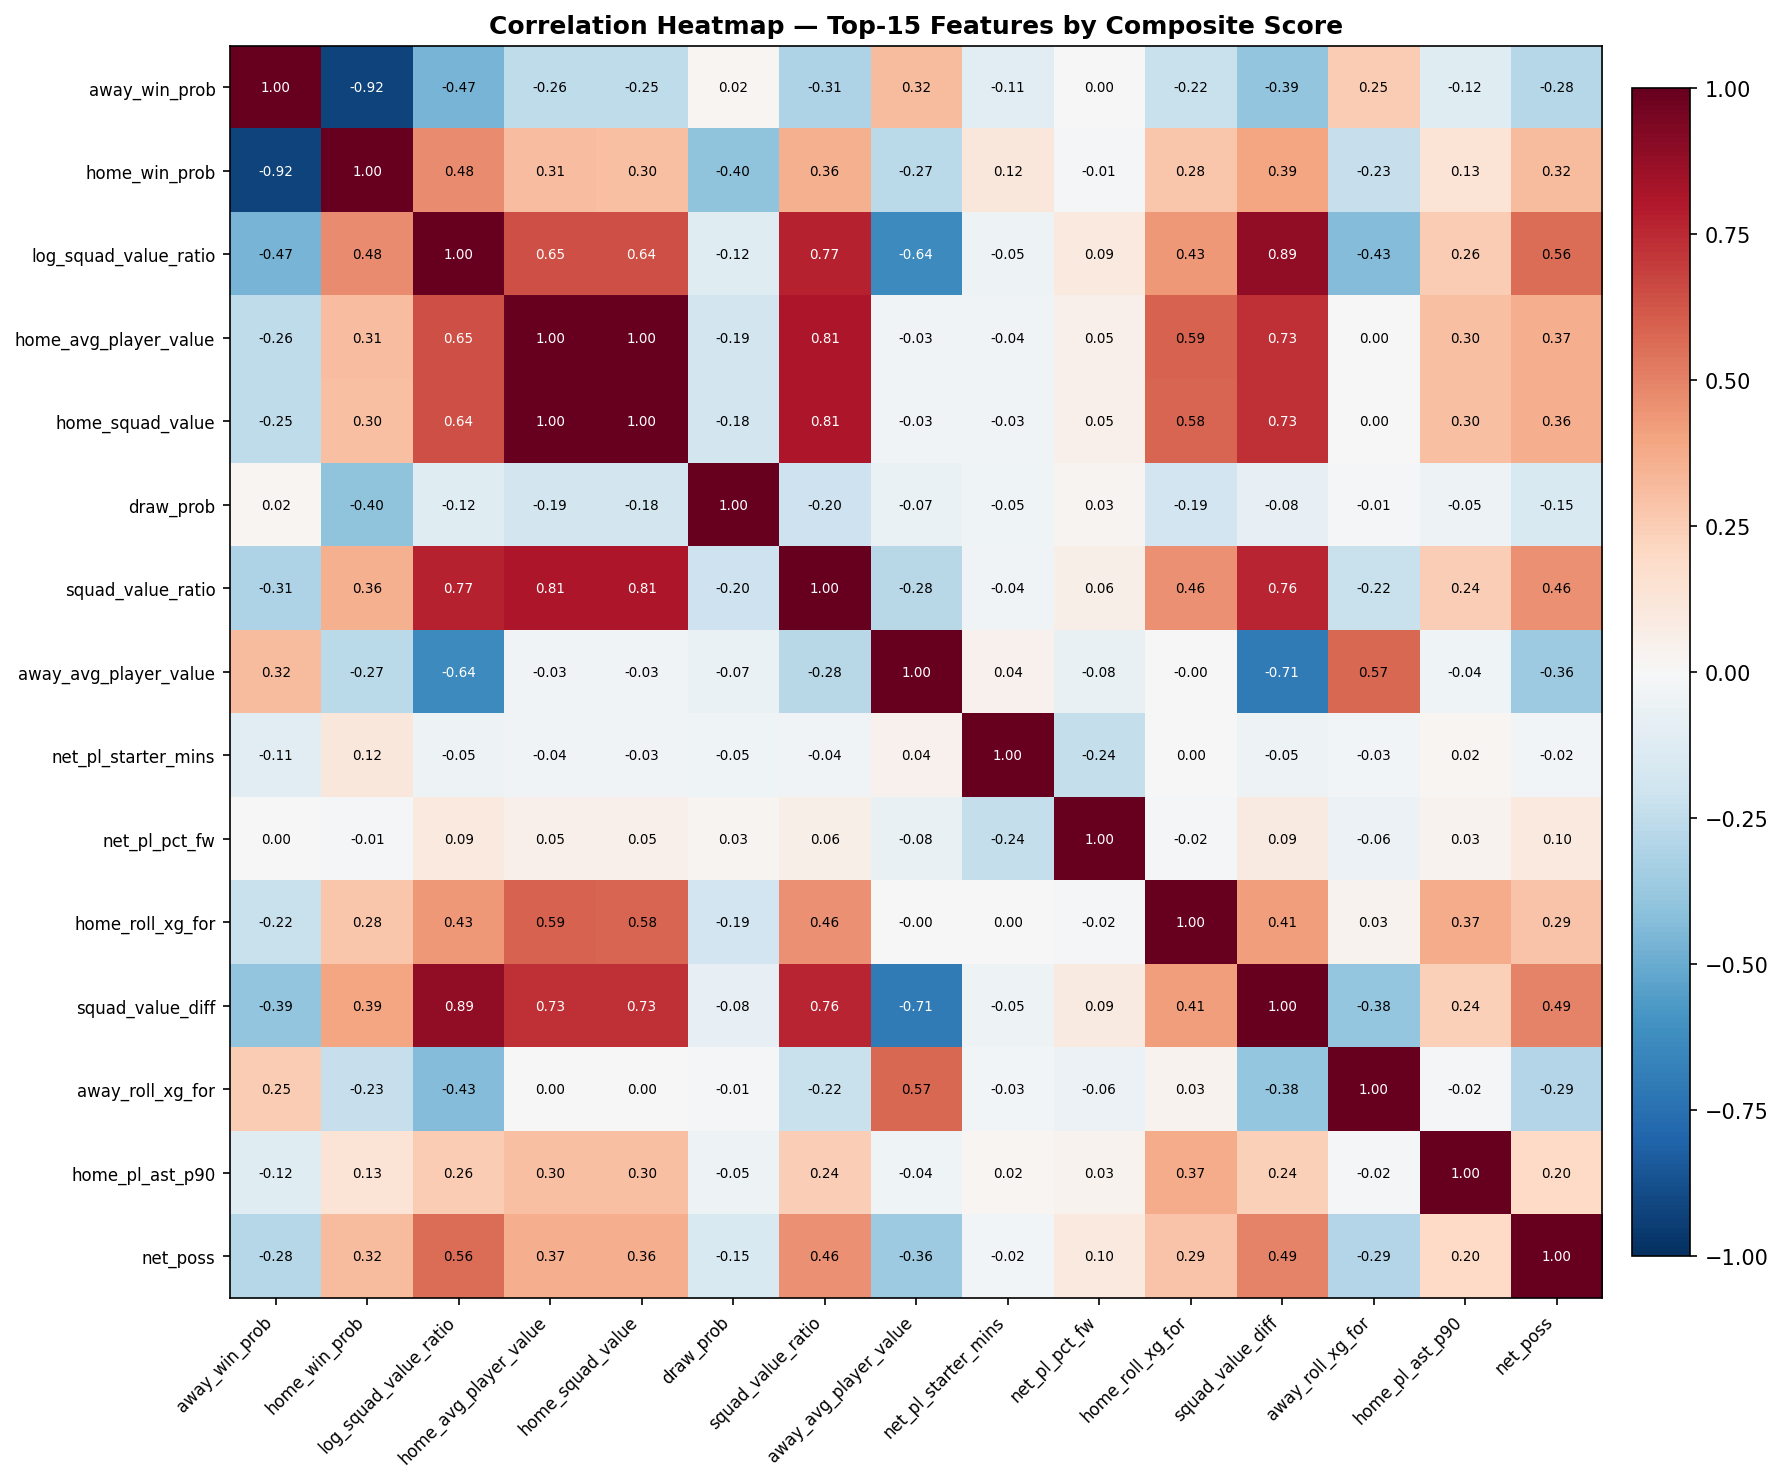
\includegraphics[width=\linewidth]{../outputs/eda/14_top15_correlation_heatmap.png}

    \column{0.45\textwidth}
    \vspace{0.5em}
    \small\textbf{Red zones} = high correlation $\Rightarrow$ redundant
    (e.g.\ \texttt{home\_win\_prob} and \texttt{away\_win\_prob} are two sides
    of the same bet).

    \vspace{0.8em}
    \textcolor{playercol}{\textbf{Player features}}
    (\texttt{net\_pl\_pct\_fw}, \texttt{net\_pl\_starter\_mins}) show
    \emph{near-white rows and columns} — barely correlated with anything
    else.

    \vspace{0.8em}
    This confirms they bring \textbf{genuinely new information}
    rather than repeating the bookmaker signal.
  \end{columns}
\end{frame}

%% ═══════════════════════════════════════════════════════════
\section{Key Findings}
%% ═══════════════════════════════════════════════════════════

\begin{frame}{Key Findings}
  \begin{block}{The data pipeline}
    \footnotesize 62{,}683 FBref player-match rows across 6 seasons, joined to Understat xG and
    Transfermarkt squad values $\rightarrow$ 73-feature, 1{,}653-match dataset
    with \textbf{zero null values} in all player rolling features.
  \end{block}

  \vspace{0.25em}

  \begin{alertblock}{Answer to the hypothesis — \textbf{Yes}}
    \footnotesize
    \textbf{Signal confirmed:}
    \texttt{net\_pl\_starter\_mins} (rank~9) and \texttt{net\_pl\_pct\_fw} (rank~11)
    survive all four selection methods.\\[0.25em]
    \textbf{Depth:} 10 player features selected by RFECV, competing directly against
    bookmaker odds and squad market values.\\[0.25em]
    \textbf{Independence:} player features are near-zero correlated with the bookmaker
    signal — they add new information, not a repeat.
  \end{alertblock}

  \vspace{0.25em}
  \footnotesize\textit{Open question: by how much do these features improve log-loss
  and Brier score beyond a bookmaker-only baseline?}
\end{frame}

\end{document}
